%!TEX program = xelatex

\documentclass{article}

\usepackage{ctex}
\usepackage{float}
\usepackage{graphicx}
\usepackage{geometry}
\geometry{left=2.5cm,right=2.5cm,top=2.5cm,bottom=2.5cm}

\title{Maple遥感数据存储系统}
\author{
    海杰文\\
    计算机科学与技术\\
    3130000656
  	\and
    蔡武威\\
    计算机科学与技术\\
    3130101796
    \and
    田黄石\\
    计算机科学与技术\\
    3130100818
    \and
    熊青城\\
    计算机科学与技术\\
    3130102348
}

\date{}
\renewcommand\figurename{图}

\begin{document}

\maketitle

\section{引言}
Maple遥感数据存储系统(下称“Maple系统”)面向企业、科研单位以及个人提供高效、可靠的遥感数据服务。由于用户日益增长并且复杂的存储以及检索需求,Maple系统将存储卫星每日不断产生的遥感数据,并且对数据进行基础处理。在此基础上,Maple提供相应接口使用户可以检索不同时间段、不同区域以及不同处理等级的数据。

\section{需求分析}
\subsection{功能需求}
毫无疑问,系统的核心是存储系统,需要连续不断地存储大量数据,具有很强的时序性。日均产生的数据量将达到10T,因而数据总量将随着时间不断增加。Maple系统将存在很长的时间,长达数十年,这就对存储数量与可扩展性提出了相应的挑战。

此外,天气预报、科学研究、城市规划、公共卫生、地图、矿物探测以及军事等等,都需要大量的遥感数据,并且他们所需求的数据的等级要求各不相同,拥有不同的特性。因而Maple系统需要具有处理大规模遥感数据的能力,对数据进行初步的加工以便用户生产更高级别的应用产品。

每一个系统都需要面向更高级别的用户,而与网络应用不同的是,在Maple系统中,交互性、即时性并没有那么重要。在面向大规模数据的情况下,网络的传输速度将成为一个非常重要的指标。用户要能在全国范围都拥有稳定、快速的数据获取速度。

\subsection{性能需求}
数据存储的长期性使得Maple系统需要存储海量的遥感图片数据,包括原始全分辨率的遥感图片,时间、日期、地区等元数据,经过处理产生的地理信息以及一些分析结果等等,都需要被存储归档。整个系统必须具有每天添加10T的能力,由于成本问题首先考虑存储10年数据,依旧存储总量将膨胀到近400PB。由于本系统的存储时间会达到数十年,系统存储必须要拥有相当的可扩展性,以便在将来扩大存储规模。

遥感图片需要各种各样的算法来对其进行处理,以此生产用户所需求的图片信息。例如天气预报需要卫星云图;城市规划需要道路、楼房、高度等信息;公共卫生则需要了解植被覆盖情况。这些都是在原图的基础上加工生产的数据,因此Maple系统需要一定强度的计算能力。而由于不同数据类型的不同数据需求,系统需要对这些数据提供不同的数据能力,而且某些数据,如天气预报所需数据需要在当天及时处理并且能够提供给用户使用。

Maple系统面对全国各个单位提供遥感数据,因而我们需要让全国各个区域的用户都可以稳定有效地访问数据中心的数据。大的数据量使得地理位置对下载速度产生了相当的影响,我们需要提出有效的解决访问解决这个问题。

\subsection{可靠性和可用性需求}
数据中心必须要拥有灾难恢复的能力,大量的时序的遥感数据作为重要的科研与工业数据不能因为突发情况丢失。但是用户访问这些数据的特点是不频繁,但是单次访问将会返回大量的数据,所以RPO与RTO的要求并不高。

\section{系统设计}
\subsection{总体框架}
Maple系统分为三个不同的层级,分别为在线存储、近线存储和离线存储。其中在线存储用于存储近两周时间内的遥感卫星数据,采用存取速度较快的存储介质进行存储。在线存储的目的主要是为了提供尽可能高的访问性能,缩短用户的数据读取延时。近线存储则用于存储近一年的遥感卫星数据,采用存取速度较慢、但支持随机访问的存储介质进行存储。近线存储主要针对的是用户访问频率较低的遥感卫星数据,通过选择速率较低的存储介质降低成本,同时提供随机访问来保证相对较低的访问延时。而离线存储则主要用于数据归档,将历史遥感影像进行保存归档,一方面作为数据备份,另一方面也提供相应业务支持,例如需要长时间范围内遥感数据的科学研究等。

三种不同的存储系统通过两种不同的数据中心实现。其中总数据中心用于离线存储,次级数据中心用于近线和在线存储,以及相关服务的提供。就地理分布而言,次级数据中心将分布在全国,数目在5个左右。次级数据中心的建设将根据卫星基站以及客户单位的分布而决定,使其尽可能靠近卫星基站以及客户单位,缩短传输耗损和延迟。总数据中心将建于远离次级数据中心、较为偏僻的位置,作为异地灾难备份,提供灾难恢复的能力。

Maple系统的总体架构如图\ref{overall}所示。数据在卫星基站接收完成,然后传送至就近的次级数据中心,最后会被传输至总数据中心进行归档存储。

\begin{figure}[H]
\centering 
\includegraphics[width=0.618\textwidth]{pic/overall.jpg}
\caption{总体架构示意图}
\label{overall}
\end{figure}

\subsection{存储介质}
因为Maple系统的存储主要分在线存储,近线存储和离线存储三个层级,所以我们将根据这三个部分分别讨论其需要的存储介质以及其存储架构设计。

在线存储的存储目标为最近15天左右的数据,将面临最多的访问请求,所以我们应该优先保证其存取速度以及数据的可靠性。因此,我们将选择SSD硬盘+RAID10的磁盘阵列做后端数据存储架构。选择原因有以下几点:
\begin{enumerate}
\item Maple系统15天可能接收并储存的数据量为150T左右,分布到每个数据中心的数据量为30T。因此算上RAID10磁盘阵列翻倍的硬盘需求,每个次级数据中心需要60T的SSD硬盘做在线存储,这一花费应该是在可承受的范围之内。

\item SSD硬盘在相比普通的SATA机械硬盘大大加快了其读取数据时的速度,而RAID10不仅通过分条技术加快了数据的写入速度,同时提供了可靠的数据恢复能力。

\item 由于Maple系统服务的需求主要面向于对相同数据读取请求次数少、并发请求量少、一次请求数据量大的特点,因此没有比要在在线存储中分两级硬盘做缓存。
\end{enumerate}

近线存储的主要存储对象是近一年内的数据,这一部分数据相比在线存储可能接收到的请求量大大减少,但是我们仍然应该对其做好准备。同时,近线存储应该提供对在线存储的请求分流能力,以及对在线存储可能发生的数据丢失的恢复能力。因此,我们选择SATA硬盘+RAID5磁盘阵列作为近线存储的存储架构。选择原因考虑以下几点:
\begin{enumerate}
\item Maple系统一年的数据量将达到3.6PB的巨大数据量,此时若选择价格高而性能优秀的SSD硬盘或者是SAS盘将带来大量的价格成本,同时考虑到近线存储的数据对写入和访问的性能要求没有在线存储那么高,因此在硬盘的选择中我们可以牺牲部分性能考虑价格更为低廉的硬盘。

\item SATA盘的价格相对SSD及SAS盘大幅下降,同时又有一定的性能,因此成为这一层级我们选择硬盘的对象,同时RAID5虽然对数据的写入读出速度没有帮助,但也提供了一定的数据恢复能力。
\end{enumerate}

离线存储主要存储的是过去所有的数据,离线存储的数据几乎不会被访问到,但我们也应该考虑数据的归档,以应对可能的长期遥感数据趋势分析的需求。同时,离线存储所在的总数据中心与以上两级所在的次级数据中心地处异地,可以应对次级数据中心可能出现的灾杯数据恢复的需求。对于离线存储,我们选择磁带作为存储介质。选择原因如下:磁带介质具有存储数据稳定不易丢失,容量大且价格低廉的优势,最适合应对Maple系统里需要长期、大量的存储需求。

同时,对于在线存储和近线存储,我们应该提供作为智能存储系统作为数据写入和读出的管理系统,可以有效地管理数据的写入和读出的调配。

\begin{figure}[H]
\centering 
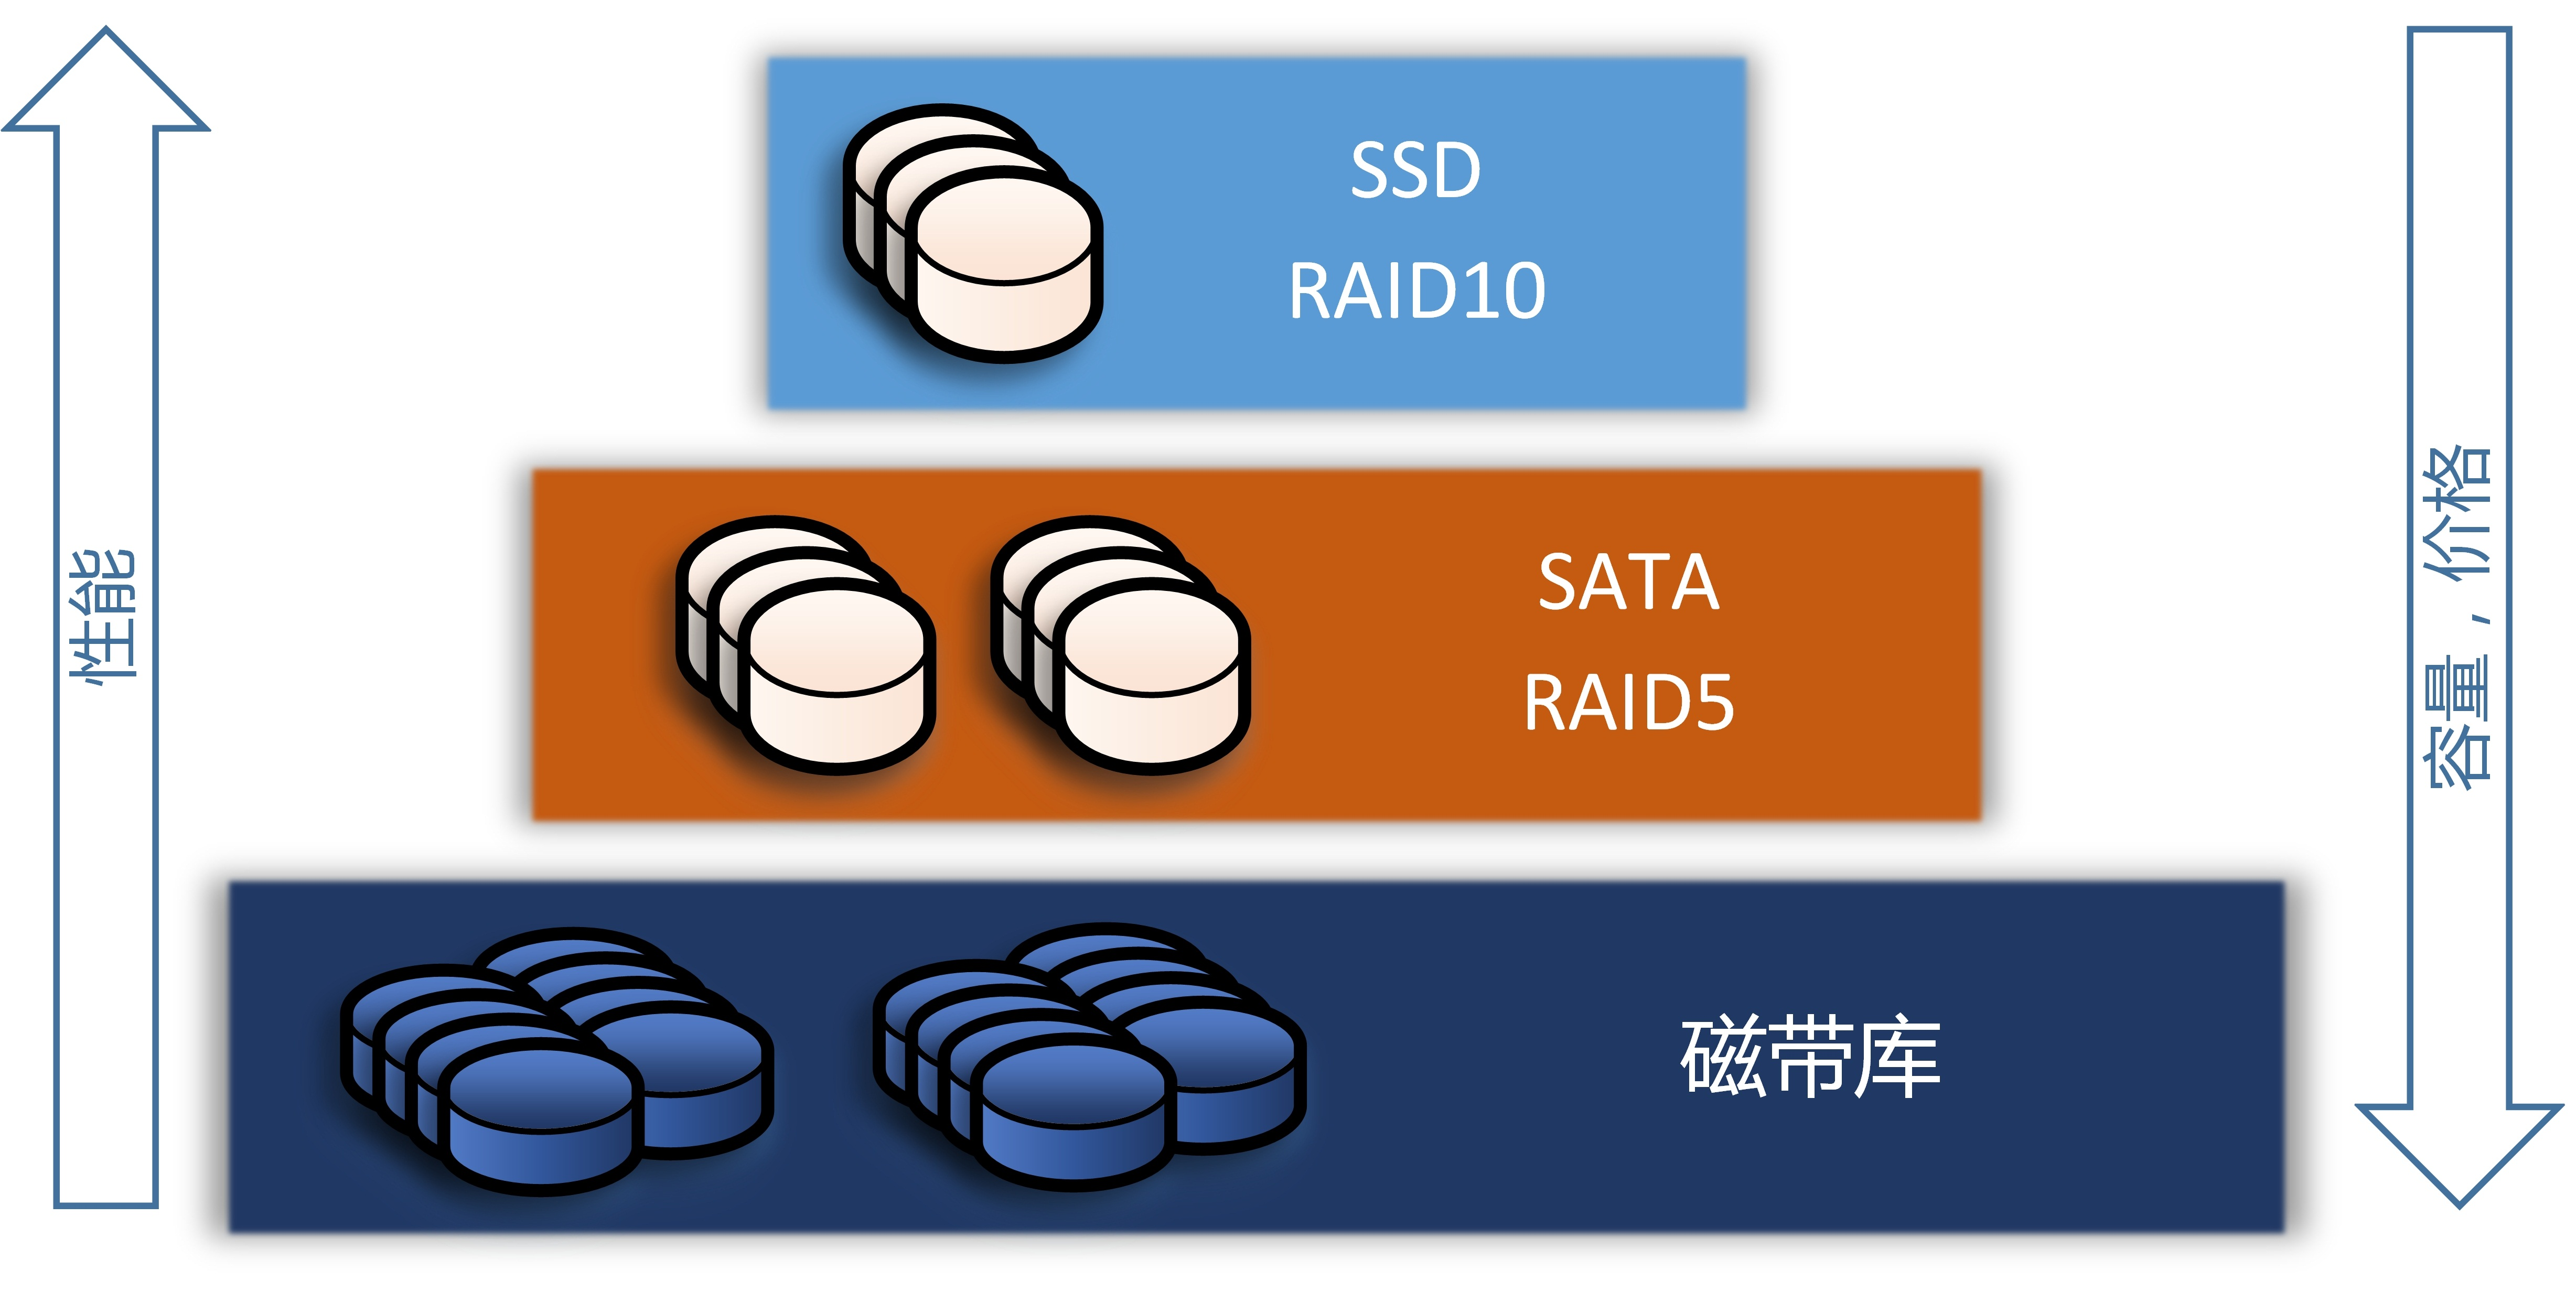
\includegraphics[width=0.618\textwidth]{pic/storage.jpg}
\caption{存储层级示意图}
\label{storage}
\end{figure}

\subsection{存储网络}
在次级数据中心内部,在线存储和近线存储将选用FC SAN进行构建。服务器与存储阵列之间通过FC网络进行连接。选用FC SAN的原因主要有:
\begin{enumerate}
\item FC SAN的具有较高的传输速度。相比起其IP SAN等其他存储网络或传统SCSI总线方式连接存储,FC SAN在传输速度上具有较大优势。并且卫星遥感数据往往涉及大量数据块的读写操作,基础存储系统构架的传输速度十分重要,因此选择采用FC SAN。
\item FC SAN具有良好的可扩展性。与传统存储阵列相比,引入存储网络可以大幅提升存储的可扩展性,为日后的业务增长提供空间。尤其对于近年来发展迅猛的卫星行业,相关业务的扩展和增长已是必然趋势,良好的可扩展性必不可少。
\end{enumerate}

次级数据中心之间以及次级数据中心与总数据中心之间将通过FCIP协议进行连接。选择FCIP的主要原因有:
\begin{enumerate}
\item 次级中心之间需要跨越不同城市,FCoE只能在以太网进行传输,无法达到如此大的跨度。而FCIP则可以利用广泛部署的IP基础架构进行远距离传输。
\item 若要直接将FC SAN相连,直接架设光缆需要投入巨大的成本。相比较而言,利用IP设备进行传输既可以利用现有的网络资源,降低建设成本,经济效益更高。
\item 由于次级数据中心出于性能考虑需要采用FC SAN,选用FCIP协议也是为了与之相契和。
\end{enumerate}

\subsection{存储系统}
Maple系统的数据量是稳定而高速增加,因此在设计之初就需要考虑到整个存储系统的可扩展性。而为了提高整体性能与降低预算,我们设计了复杂的三层结构,这加大了与存储有关的复杂性。因此文件虚拟化将被引入,并且凭借它来整合整个存储系统。我们使用多台服务器集群来将计算资源与存储资源分离开来,在文件虚拟化这一层不仅仅需要管理存储资源的动态分配,还需要管理数据迁移与归档。上层的数据处理服务器与数据分发服务器则不需要关心底层的文件是在哪个数据中心的哪一个磁盘上,仅需要从一个统一命名空间的文件系统中获取数据即可。

\subsection{计算平台}

Maple系统作为一个完整的遥感数据处理系统,需要一个支撑平台能够提供计算能力来处理其海量的遥感图片数据。为了让整个系统拥有良好的灵活性与更高的可用性,拥有快速更新技术、更快调配IT资源的能力,我们将为整个系统引入云的概念。

根据我们之前的设计结构,首先分析三层存储结构的特性。在线存储与近线存储被放在次级数据中心与卫星基站处在同一位置,负责接收、处理遥感数据而且承担主要的图片数据传输服务,而离线存储则被放在总数据中心,辅助提供数据传输服务,并作为灾备的主要手段。从这个结构可以看出,整个系统是以存储为中心的,计算则主要集中在次级计算中心。持续不断的图片处理需要强大的计算量,因此我们将在每个次级数据中心的硬件基础上建立私有云,以方便数据中心的管理与扩展。在私有云之上部署有Hadoop集群处理图像数据,此外,大量的Web服务器也被部署在这个平台上用于处理数据请求。次级数据中心构架如图\ref{sub}所示。

\begin{figure}[H]
\centering 
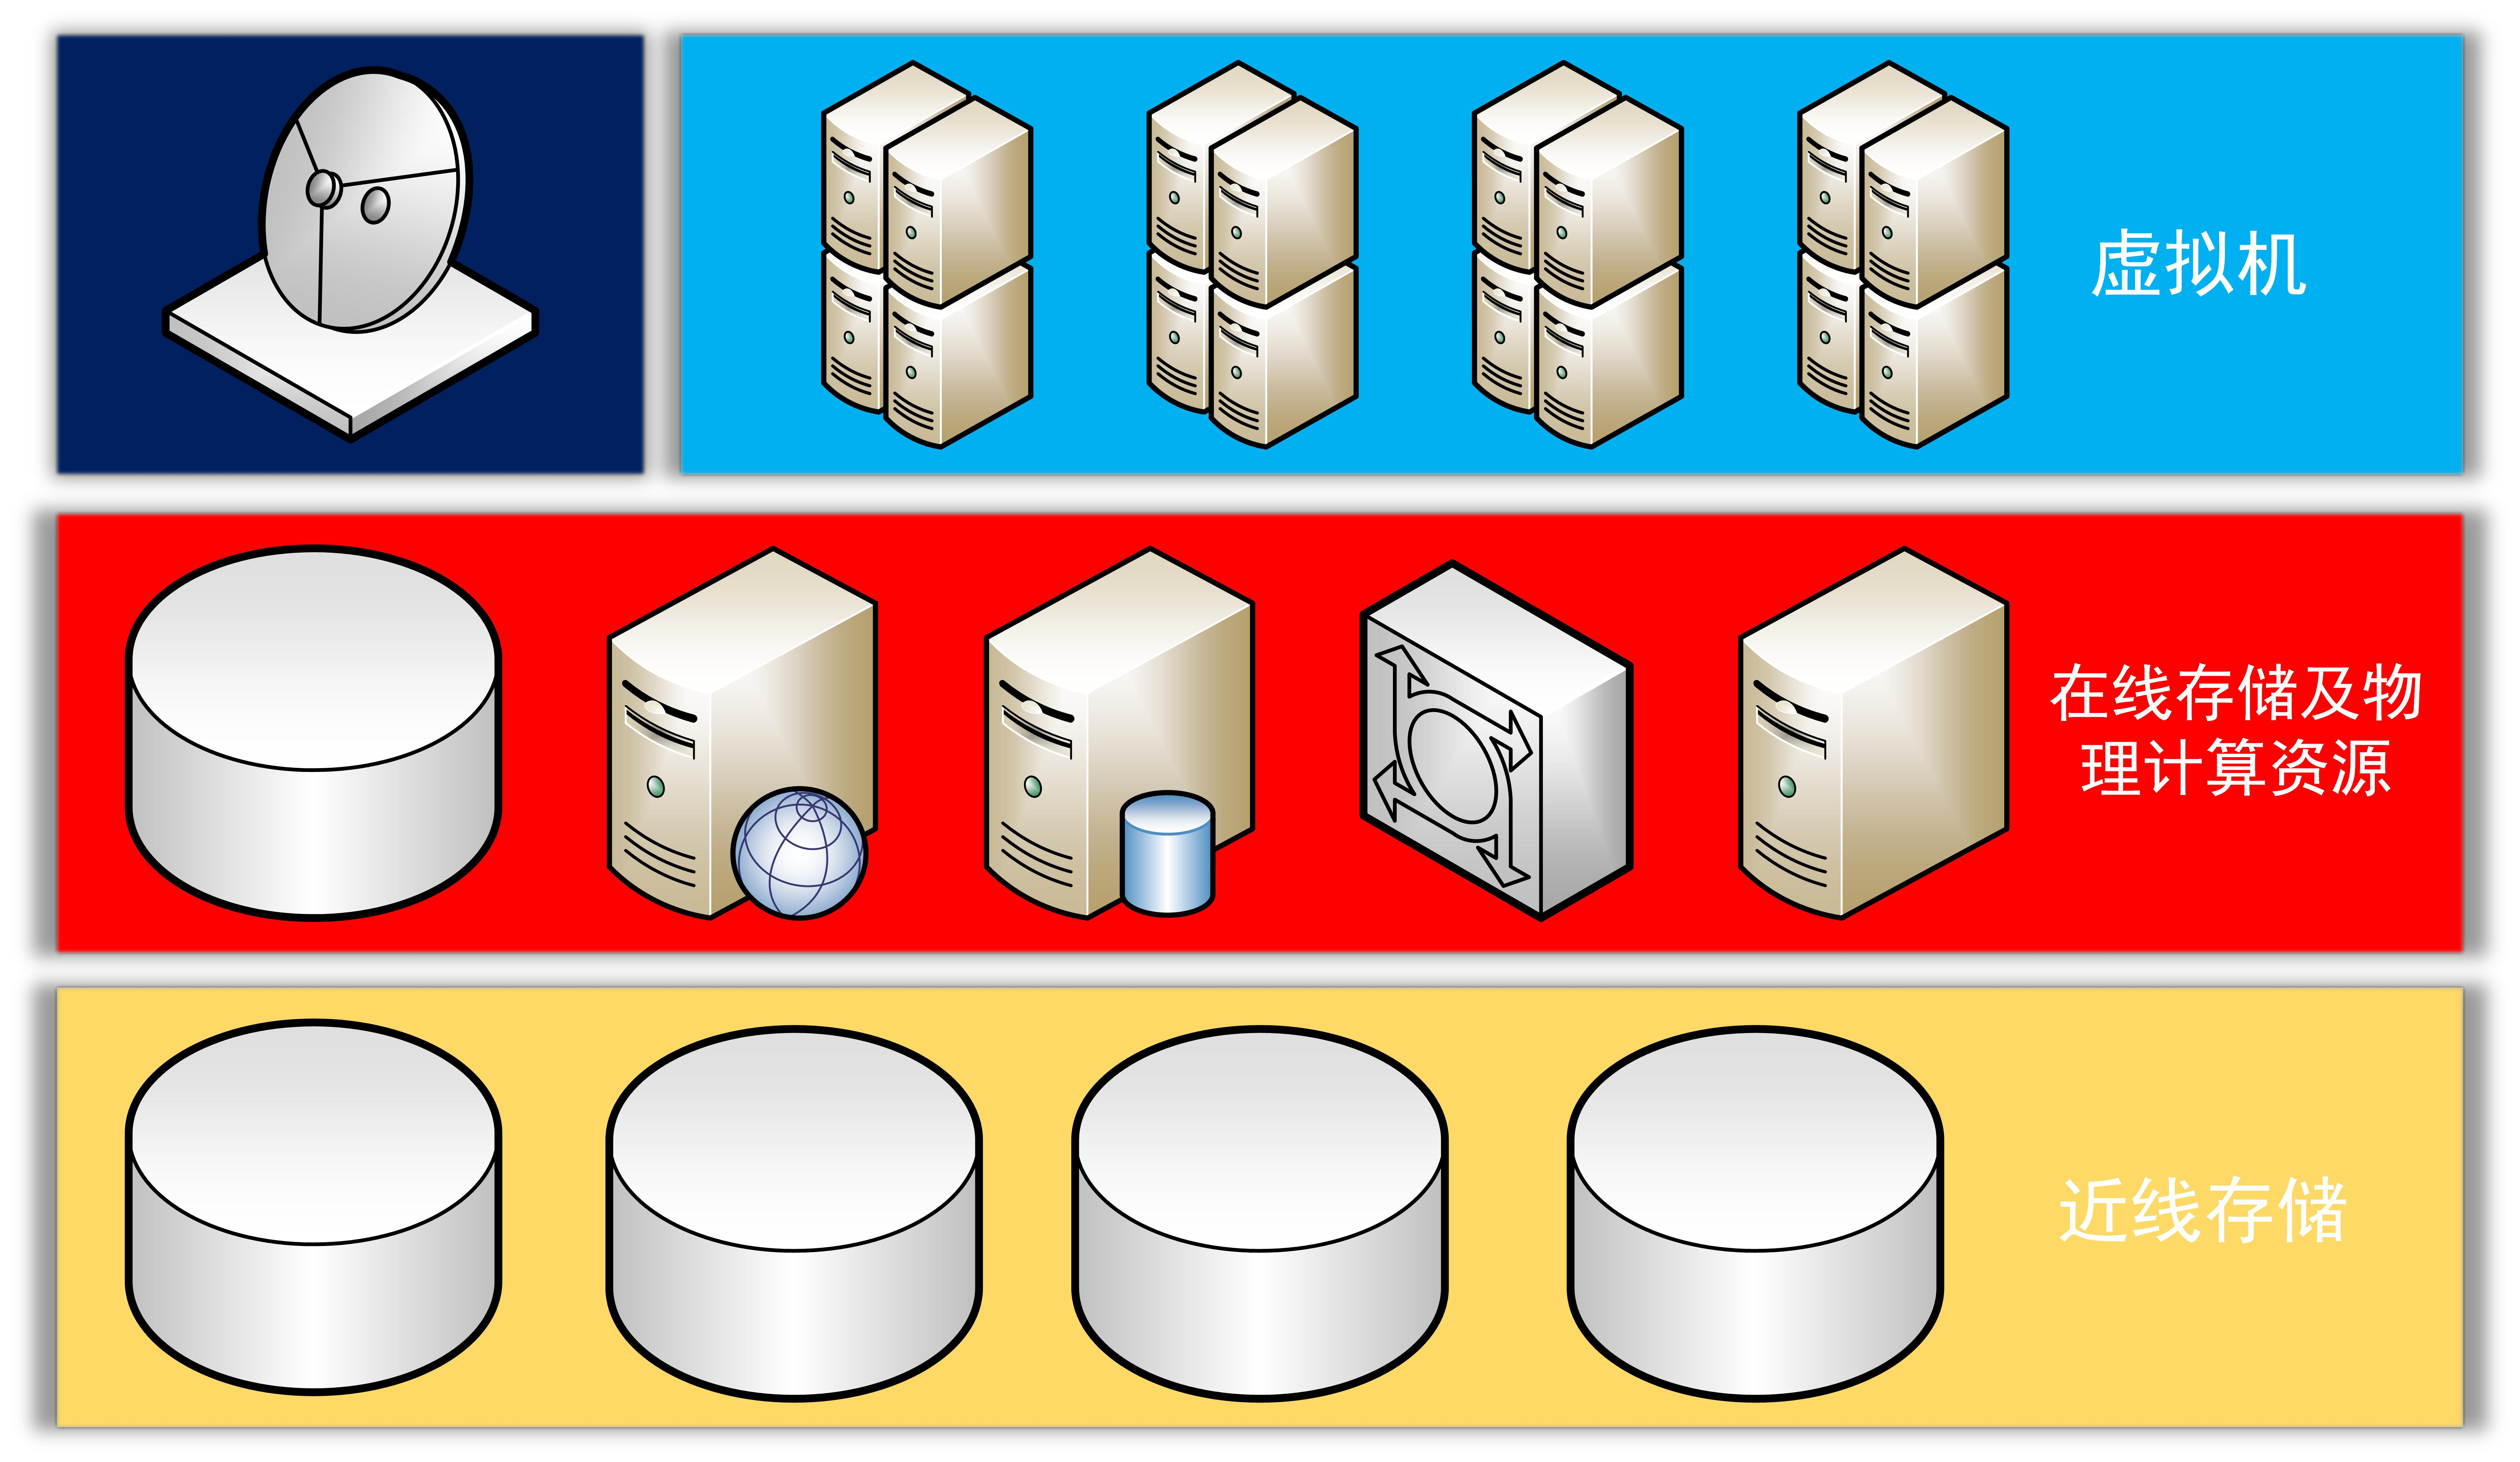
\includegraphics[width=0.618\textwidth]{pic/sub.jpg}
\caption{次级数据中心架构示意图}
\label{sub}
\end{figure}

每个数据中心的基础计算能力都由大量普通的Linux服务器组成,在这些服务器之上将安装kvm以提供虚拟化能力。使用OpenStack作为中间件,从而虚拟化出大量的虚拟机供平台部署应用。在这之上我们将配置完整的应用运行环境,进而将图像处理的应用实例部署在每一台虚拟机上。整个数据中心的计算资源已经被统一管理,所以Web应用程序还有内容管理系统都可以被部署在这个平台上面,这样平台的可扩展性与业务灵活性的要求就被满足了。而总数据中心主要负责归档,使用大量的磁带机以满足海量数据的存储需求,对计算资源并没有很多需求,仅需要满足不频繁的数据检索即可。

\subsection{数据迁移}
Maple系统的数据量使得数据迁移成为一个非常值得注意的问题,而从数据处理到归档的整个过程有大量的数据的流动,而其主要则是数据的归档。我们所设计的系统必须能够很好地处理极大规模数据的,从而提升整个系统的性能。整个Maple系统的数据迁移分为两个部分,数据中心内部的数据流动和数据中心之间的数据传输,对应了两个层次的数据迁移与复制,即本地复制以及远程复制。考虑Maple系统的结构,所有计算都集中在卫星遥感数据传输完成后的图像处理上。这里的计算负载是非常巨大的,而之后则是不断的归档与存取过程,几乎不会对数据产生任何修改。因此在数据迁移上,我们就只需针对这种一次计算、多次归档的性质进行设计。

由于引入了文件虚拟化,数据迁移对于上层来说相对透明,本地复制仅由虚拟化应用装置完成即可。在虚拟化层之下,因为整个系统需要不断向下级存储介质不断写入,将采用基于指针的完整卷复制作为本地复制的方式,并且采用完整拷贝模式。这种模式对源的性能影响最小,并且支持立即访问。

同样,两个数据中心之间的数据迁移也由于文件虚拟化的引入变得透明了许多。通过我们已经建立好的FCIP将虚拟卷进行复制即可。Maple系统对于RPO的要求不高,使用每级存储之间采用异步的远程复制就可以满足我们归档的需求。

整个Maple系统拥有5个次级数据中心与2个总数据中心,他们互相之间的调度将非常复杂,由上层的应用服务器处理这些问题将会变得非常难以管理因而降低可扩展性。所以这些复杂的调度都由一个专门的数据迁移管理模块进行管理,在统一管理之下,上层就不需要关心复杂的备份机制,而只需要处理好业务即可。数据迁移管理模块将管理整个系统的数据迁移、备份的策略,主要备份策略将在下一节说明。

\subsection{数据备份}
Maple 系统要向各类客户提供高效、可靠的遥感数据服务,并且提供相应接口为用户提供可以检索不同时间段的数据的服务。考虑到客户的需求和Maple系统的时效性,Maple系统将一直处于运行状态,因此Maple系统必须采用热备份的策略。

在备份粒度上,由于Maple系统的数据庞大,以离线存储尤为明显,完全备份的代价超出了可承受的范围;同时Maple系统是一个可靠的系统,数据恢复的频率要远低于数据备份的频率,因此采用增量备份的策略。与累计备份及恢复相比,增量备份及恢复的策略备份所用的时间更少、需要的存储空间更少而恢复时间更长。前两者有助于节约Maple系统的存储成本并提高Maple系统的效率,而恢复时间更长的劣势在这一恢复频率较低的系统中并不突出。

Maple系统拥有在线存储、近线存储和离线存储三个不同的层次,且在线存储的数据会不断复制到近线存储,同时近线存储的数据也会不断传向离线存储,可以将近线存储和离线存储中的数据视为在线存储的备份,把离线存储中的数据视为近线存储的备份。上层存储结构向下层存储结构传输数据的过程的同时也可以视作是一个备份的过程。因此也可以用离线存储的数据进行近线存储的数据的恢复,用离线存储或近线存储的数据进行在线存储的数据恢复。因此,离线存储的数据安全性必须得到保证。

离线存储采用磁带备份的策略,主要由于磁带备份是一种传统低成本的备份方案,而离线存储中数据量是极大的,这可以大大减少Maple系统的成本。 为了提高备份的效率和介质的性能,这一磁带备份可采用多数据流的方式备份。处于灾难备份的考虑,离线存储拥有两个处于异地的数据中心,每一数据中心都存有离线存储的备份。总数据中心如图\ref{all}所示。

\begin{figure}[H]
\centering 
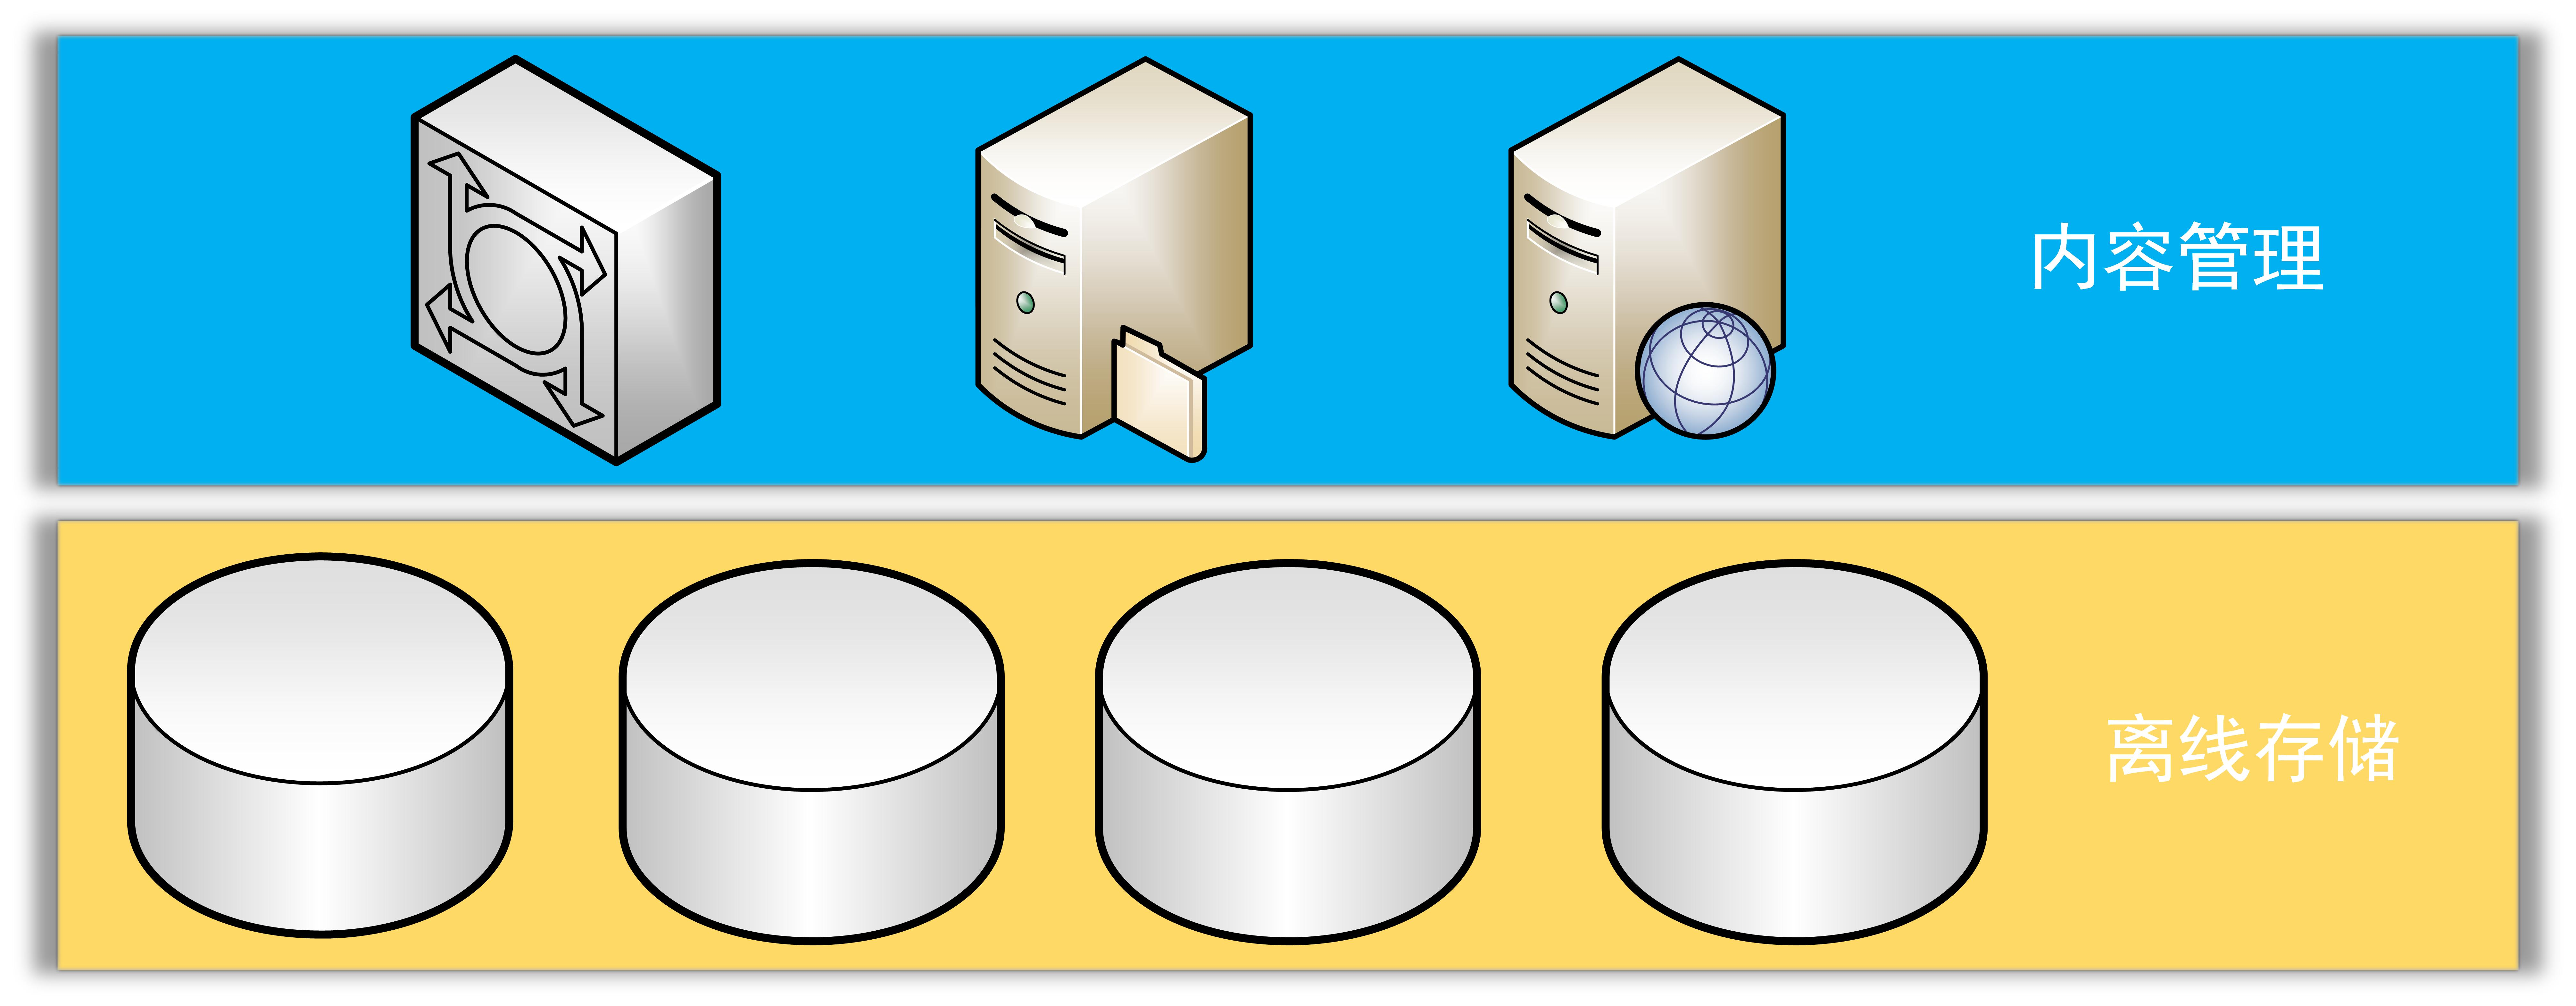
\includegraphics[width=0.618\textwidth]{pic/all.jpg}
\caption{总数据中心架构示意图}
\label{all}
\end{figure}

\section{总结}
整个Maple系统提供了一个SaaS级别的遥感影像检索服务,主要面对企业与科研单位等专业用户。持续不断的数据增长以及告诉增长的遥感数据产生速度对存储及计算的可扩展性产生了极大的需求,而大数量的遥感数据检索服务则对数据访问速度产生了挑战。通过虚拟化技术,我们成功解决了计算能力的可扩展性,三层存储结构则在较低成本下提高了用户的体验。

\begin{figure}[H]
\centering 
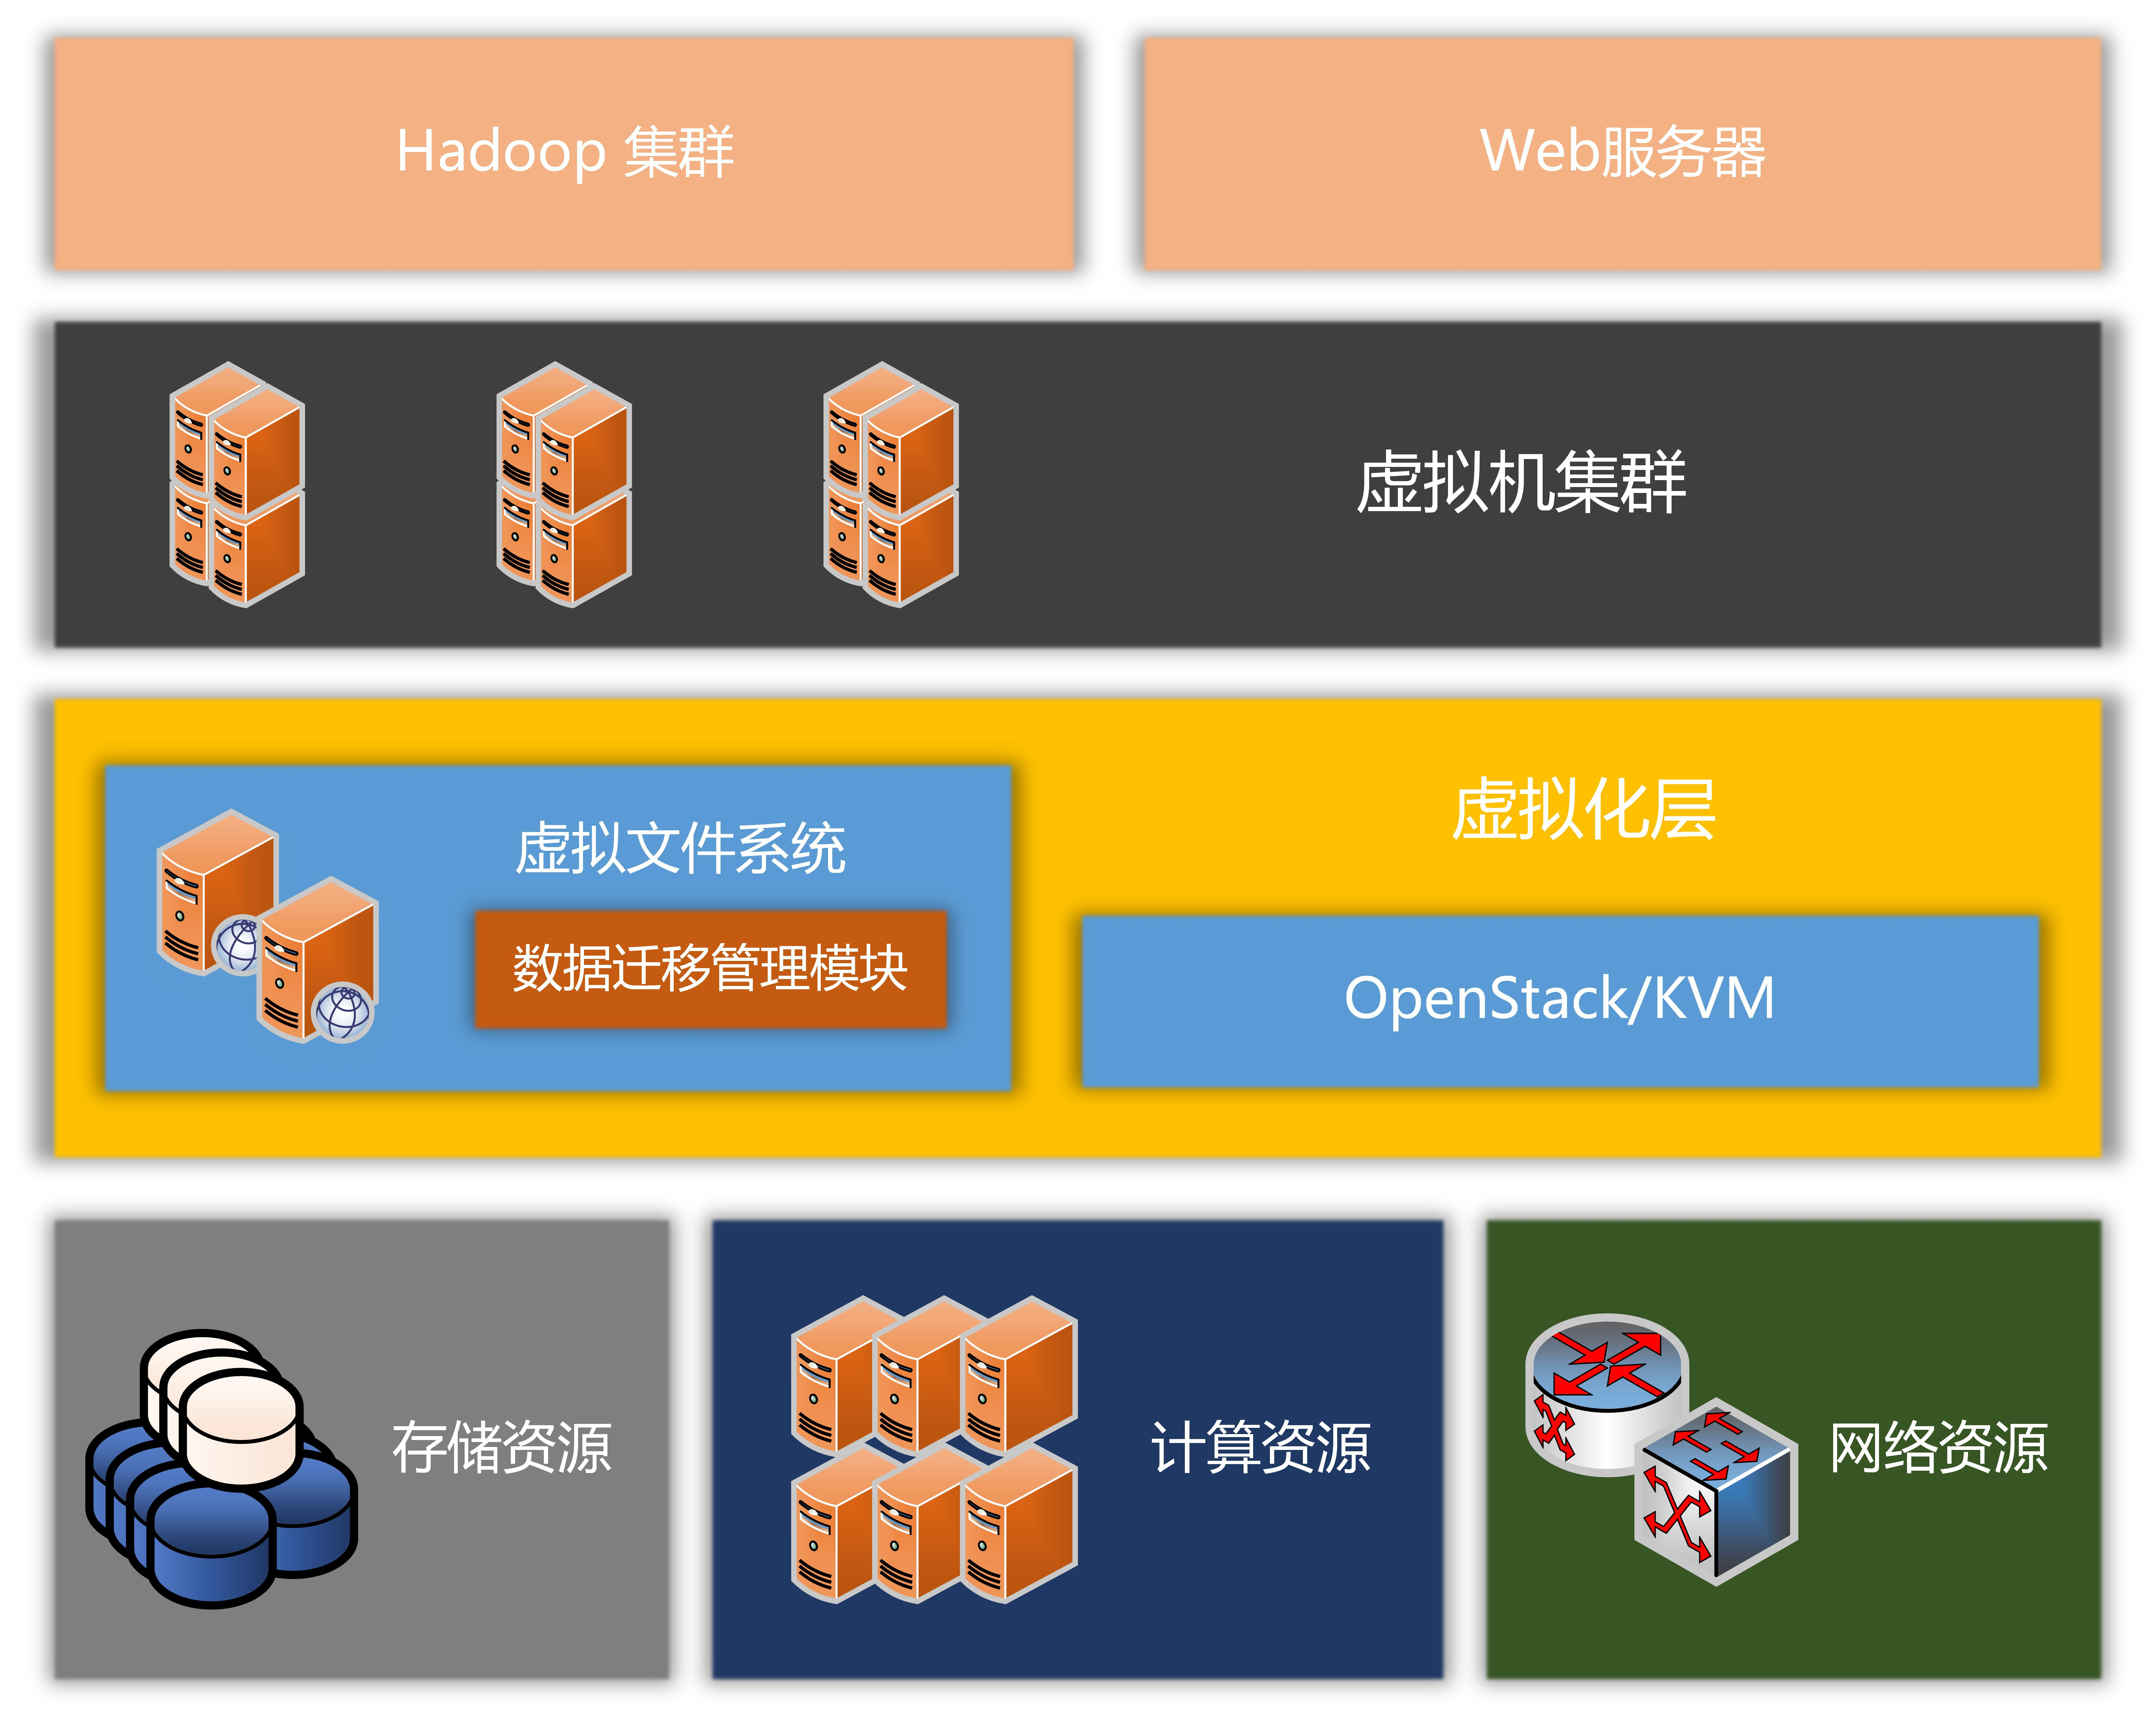
\includegraphics[width=0.618\textwidth]{pic/logic.jpg}
\caption{Maple系统逻辑架构示意图}
\label{logic}
\end{figure}

\end{document}